\section{Introdução}

Linguagens de programação interpretadas tem sacrificado performance
em favor de um alto nível de abstração do funcionamento da máquina
envolvida, possibilitando maior expressividade, facilidade de
desenvolvimento, portabilidade, flexibilidade, dinamicidade, entre outros.
Especificamente a linguagem de programação \texttt{Tcl}
(\textit{Tool Command Language}), teve como um de seus maiores
objetivos a facilidade de incorporação (\textit{embedding}) a
programas que desejassem ter uma linguagem de comandos
\cite{ousterhout_89}. Uma interface simples e extensível para
aplicações em linguagem \texttt{C} era o fator motivante de seu uso.
Programas inteiramente em \texttt{Tcl} eram vistos como pequenos
scripts, muitos talvez de uma linha no máximo \cite{ousterhout_89}.
Entretanto, aplicações em \texttt{Tcl} com milhares de linhas,
como por exemplo exmh \cite{exmh}, OpenACS \cite{openacs} ou mesmo a
suíte de testes do GDB (\textit{GNU Debugger}) \cite{gdb_testsuite},
tem surgido e a reescrita de trechos críticos em \texttt{C} vem sendo
aplicada para reduzir o impacto da máquina virtual no tempo de execução.

Outra forma de melhorar o desempenho de linguagens e, portanto,
reduzir a necessidade de reescrita de código em linguagens compiladas,
é através da utilização da compilação JIT (\textit{Just-In-Time}) que
realiza tradução de código sob demanda. No caso desse trabalho, estamos
interessados na tradução de \textit{bytecodes} da máquina virtual
\texttt{Tcl} para código de máquina durante o tempo de execução.
Informações acerca do programa em execução são coletadas
conforme necessário para dirigir a compilação dinâmica. Portanto,
linguagens tipicamente difíceis de serem analisadas e compiladas
estaticamente, devido a uso de, por exemplo, tipagem dinâmica ou
escopo dinâmico, ganham a oportunidade de melhoria de desempenho
com uso de tal sistema de compilação.

O trabalho presente pretende melhorar o desempenho da linguagem
\texttt{Tcl}, reduzindo o tempo de decodificação e interpretação
de \textit{bytecodes} através da implementação e implantação de um
compilador JIT na mesma. Diversos trabalhos, como
\cite{deutsch84efficient} para a linguagem \texttt{Smalltalk},
Jalapeño \cite{jalapeno_1} para \texttt{Java}, Psyco \cite{psyco}
para \texttt{Python} ou a implementação do SELF-93 \cite{holzle},
demonstraram resultados bastante significativos ao implantar tal
método de compilação. Pretende-se ainda manter um nível de
manutenibilidade e flexibilidade adequado, permitindo extensões e
futuro desenvolvimento sobre esse trabalho inicial.

Um compilador JIT requer que as estruturas internas sejam
suficientemente eficientes, caso contrário não se torna viável o
uso de um compilador otimizador em tempo de execução. As escolhas a
cerca de quais representações intermediárias utilizar, como estruturar
os dados, quais otimizações aplicar e algoritmos para diversas fases da
compilação, devem ser feitas de forma a conseguir balancear baixo
tempo de compilação com código gerado de alta qualidade. Ainda há o
quesito de consumo de memória principal, que, apesar da crescente
capacidade disponível, geralmente costuma ser um recurso escasso em
dispositivos embarcados. Sabe-se que o interpretador \texttt{Tcl} está
presente em roteadores da Cisco, pois vem incluso no Cisco IOS
(\textit{Internetwork Operating Systems}), mas esse trabalho
não tem como foco tal tipo de dispositivo e, portanto, consumo de
memória não será um dos pontos levados em consideração. Porém, entre
os fatores complicadores consideramos também a manutenabilidade do
sistema. Um nível muito alto de abstração, como dito no ínicio do
texto, impediria a utilização de um programa de desempenho crítico e,
por outro lado, um nível muito baixo dificultaria a correção/detecção de
problemas e melhorias gerais.
Uma alternativa para esse problema vem sendo aplicada através do
projeto PyPy \cite{pypy}, onde um interpretador para uma linguagem
qualquer é escrito em \texttt{RPython} (uma implementação mais
restrita da linguagem \texttt{Python}) e o PyPy realiza a tradução do
mesmo para a
linguagem \texttt{C} incluindo (atualmente) juntamente um compilador
JIT específico para arquitetura IA-32. Entretanto, um
dos objetivos do trabalho discutido aqui é analisar como um sistema de
tamanho reduzido compete com sistemas mais robustos. Não se tem a
intenção de fornecer um ambiente de alto nível para construção de
outras máquinas virtuais com ou sem compiladores JIT para
\texttt{Tcl}, mas sim uma implementação específica e direta.
A escolha da
linguagem \texttt{C} reflete esse objetivo porque não adiciona novas
dependências ao núcleo da linguagem \texttt{Tcl} além de ser
considerada bastante eficiente.

Procura-se visar a simplicidade, de forma que o trabalho desenvolvido
possa servir de base para expansão a novas arquiteturas e também para
aplicação de técnicas de compilação diversas sob a
\texttt{Tcl}. Na representação intermediária quádruplas são
escolhidas para formar blocos básicos e
esses, por sua vez, são utilizados para definir grafos de fluxo de
controle que servem de entrada a outra representação escolhida -- SSA
(\textit{Static Single Assignment}). A arquitetura IA-32 foi escolhida
como alvo, pois está presente em boa parte dos computadores de uso
pessoal, porém a linguagem \texttt{Tcl} atualmente executa em várias
outras arquiteturas. Nesse sentido, permitir portar para IA-64, ARM, e
outras, sem tornar a tarefa demasiadamente complicada faz parte da
simplicidade que se pretende práticar.

A seção \ref{rev_biblio} realiza uma revisão bibliográfica relevando
trabalhos que, de alguma forma, buscaram melhorar a performance da
\texttt{Tcl}. Também descrevemos brevemente alguns projetos de
compiladores JIT que apresentam alguma semelhança com o nosso. Em
seguida, na seção \ref{proposta} é descrito uma proposta um pouco mais
detalhada a respeito desse compilador. Na seção \ref{desenvolvimento}
alguns detalhes do que já foi desenvolvido são apresentados, incluindo a
estrutura atual para quádruplas e blocos básicos. As demais seções
se destinam a mencionar dificuldades encontradas até qui, além de
descrever o que será feito a partir desse ponto.


\section{Revisão Bibliográfica}
\label{rev_biblio}

A linguagem \texttt{Tcl} já obteve ganhos de performance em diferentes
estudos feitos. Um deles, que atualmente faz parte da implementação da
linguagem, descrito em \cite{tcl_bytecode}, é a geração e a
interpretação de \textit{bytecodes}. Anterior a esse trabalho, foi
demonstrado em \cite{sah_tc} que o \textit{parsing} do código
realizado a todo momento para sua reinterpretação e também a conversão
excessiva entre tipos de dados, pois a \texttt{Tcl} trata tudo como string,
eram os grandes consumidores do tempo de execução. Com esse trabalho
feito, a linguagem passou a utilizar representação dupla para os
valores presentes na execução do programa. Uma representação é
interna, possivelmente mais eficiente para se trabalhar. A outra é a
típica representação em string que a linguagem sempre usou. Caso uma
delas não esteja disponível, a outra é utilizada para recriar essa
representação se necessário.

Um trabalho mais recente, descrito em \cite{vitale_catenation}, lida
com a eliminação do \textit{overhead} de decodificação dos
\textit{bytecodes}, introduzido pelo trabalho descrito anteriormente,
fazendo uso de \textit{templates} que contém as instruções em
código nativo utilizadas para interpretar cada \textit{bytecode}.
Esse código é obtido através da compilação do próprio interpretador
\texttt{Tcl} e cada \textit{template} é copiado múltiplas vezes,
numa área de memória alocada em tempo de execução, conforme a quantidade de
cada \textit{bytecode} gerado. Nesse trabalho o interpretador foi
modificado de forma a sempre executar somente tal código formado por
uma concatenação de \textit{templates}, eliminando o \textit{overhead} de
decodificação. Demonstrou-se que em certos testes o desempenho da
linguagem pode melhorar em até 60\% com a aplicação dessa técnica.
Esse trabalho é provavelmente o mais próximo, quando considerando
somente a \texttt{Tcl}, do que se pretende produzir aqui.
Ele não gera código, mas cópia código já gerado por um compilador
estático e replica conforme necessário, fazendo os devidos
ajustes, em tempo de execução. Por um lado o tempo de ``compilação'' é
bastante baixo, porém, não dá espaço para técnicas de otimização e assim
limita o potencial de melhoria de desempenho.

Outros trabalhos, para diferentes linguagens, se assemelham mais com a
proposta aqui discutida. A busca por máquinas virtuais de alta
performance tem, atualmente, se dirigido principalmente a linguagem
\texttt{Java}. É comum a presença de compiladores JIT em máquinas
virtuais para essa linguagem, cada um com diferentes
características. A JUDO \cite{judo}, faz uso
de compilação dinâmica com dois tipos de compiladores e coleta
informações em tempo de execução. O primeiro desses compiladores é um
mais simples, que gera código rapidamente, destinado a compilação
de métodos invocados pela primeira vez. O segundo compilador é
utilizado quando informações coletadas indicam que certos métodos
são executados muito frequentemente e, portanto, estes podem se
beneficiar com a aplicação de otimizações. Essa recompilação dinâmica
é feita com o intuito de balancear o tempo gasto na compilação com o tempo
efetivamente gasto na execução do programa. Esse sistema trabalha com
a compilação de métodos por inteiro, assim como o trabalho proposto
aqui. Enquanto isso, o trabalho discutido em \cite{suganuma_pldi_2003}
avalia a aplicação de compilação dinâmica a regiões de código, evitando
a compilação de trechos raramente executados. Além disso, esse sistema
utiliza um modo misto de execução, onde interpretação e execução de
código nativo se alternam. Nesse ponto, nosso trabalho e aquele em
\cite{suganuma_pldi_2003} se assemelham.

Nos dois trabalhos sobre JIT mencionados acima não há uma descrição
a cerca das representações intermediárias (IR) utilizadas. Porém, um
outro trabalho
apresentado sobre a JVM (\textit{Java Virtual Machine}) CACAO \cite{cacao},
descreve algo parecido com a nossa proposta. De forma semelhante com a
``TVM'' (\textit{Tcl Virtual Machine}), a JVM tem uma arquitetura de
pilha e a CACAO faz uma conversão para uma representação orientada a
registradores com uso de poucas instruções. O artigo por
\citeonline{suganuma_ibm} vai além, exibindo a evolução de uma JVM
desenvolvida na IBM onde, inicialmente, era utilizado uma IR baseado
em pilha, porém mais compacta que a representação em \textit{bytecodes} da
\texttt{Java}, e que mais tarde passou também a se basear em
registradores. Os autores argumentam que para conseguir balancear
performance e tempo foi necessário, além de outros avanços, fazer uso
de 3 representações: aquela que já existia (chamada de EBC --
\textit{Extended Bytecode}) e de mais duas baseadas em
registradores. Cada uma delas recebe um conjunto de otimizações, sendo
feito propagação e cópias de constantes, eliminação de código morto,
eliminação de verificação de exceção, e algumas outras, enquanto que na
forma de quádruplas. A última dessas aparece na forma SSA, com os nós
sendo formados por quádruplas (assim como o compilador proposto aqui fará).


\section{Proposta}
\label{proposta}

Para chegar ao código de máquina final, esse projeto se propôs em
primeiro momento estudar e definir qual subconjunto da linguagem poderia
se beneficiar mais com tal técnica. O subsistema de Entrada/Saída, por
exemplo, dificilmente ganharia em desempenho com compilação dinâmica
uma vez que o tempo gasto para transferência e aguardo por dispositivos
costuma ser muito maior que o tempo das outras operações envolvidas.
Por outro lado, operações aritméticas podem ser bastante favorecidas.
O trabalho feito no Psyco, mostra melhoria
de 109 vezes no tempo de execução para aritmética de inteiros e 10,9
vezes em aritmética de ponto flutuante \cite{psyco}. Após essa
primeira análise, ve-se que entre todos os
\textit{opcodes} definidos cerca de 100 deles são de
uso geral, enquanto que o restante é dedicado a alguns poucos comandos
pré-definidos. Além disso, por volta de 20 deles realizam a mesma
tarefa mas trabalham com operandos de tamanhos diferentes (1 ou 4
bytes). Também encontramos que dois \textit{opcodes} são obsoletos,
reduzindo um pouco mais o subconjunto de trabalho.

Em paralelo ao requisito acima, foi iniciado o projeto e
implementação de uma representação intermediária de baixo
nível. Num primeiro momento sugerimos utilizar um conjunto reduzido de
instruções (RISC), assim como é feito na GNU lightning \cite{gnu_lightning},
para construir uma
árvore de instruções mais próximas da máquina alvo. Parte dessa
decisão inicial ainda se mantém, o uso de algo parecido com RISC, mas
partimos para uso de quádruplas seguida da representação SSA.
A escolha inicial por árvores foi devido
a existência de diversos métodos para seleção de
instruções que trabalham sobre essa forma de representação
\cite{ir_tree_parsing}, mas trabalhar com quádruplas se mostrou
bastante simples. O sistema de compilação dinâmica precisa ser
capaz de determinar quando iniciar e parar a construção dessas
representações.
Nesse projeto a intenção é fazer uso dos
limites de um procedimento como pontos de inicio e parada. Ainda aqui,
é importante que o sistema colete informações, como de tipos
utilizados, necessárias de forma a simplificar o código gerado, para
que não repliquemos os resultados do trabalho feito em
\cite{vitale_catenation}.

Após essas etapas pretende-se aplicar pelo menos algumas das
otimizações clássicas tais como remoção de código morto, propagação de
constante e movimentação de código.

Chegamos, assim, na fase de seleção de instruções
seguida de alocação de registradores. Há diversos algoritmos, como
\textit{Maximal Munch}, seleção com uso de programação dinâmica ou
NOLTIS \cite{noltis}  para seleção de instruções além de vários
outros, por coloração de grafos ou mesmo através de uma varredura
linear \cite{linear_scan_regalloc} (com ou sem \cite{wimmer_franz}
desconstruir a representação SSA), para alocação de registradores.
Ainda não está decidido quais dos algoritmos serão aplicados nesse
projeto, porém as metas são duas: que a implementação permita utilizar
diferentes algoritmos e que o tempo gasto para execução deles
seja compatível com um sistema que consome tempo de execução do programa.

Finalmente temos a geração de código. O foco desse trabalho é a
arquitetura IA-32, que possui uma ampla quantidade de instruções, extensões e
diversas formas de endereçamento.
Porém, não pretendemos fazer uso de todos os recursos disponíveis de
forma a tornar factível a criação do gerador.
Idéias e trechos de trabalhos anteriores, como Harpy \cite{harpy}
ou o \textit{Tiny Code Generator} (incluído nas versões mais recentes do
QEMU \cite{qemu}), podem ser reutilizadas aqui.
Ainda, de forma semelhante com a etapa anterior, a infraestrutura
permitirá a implantação de geração de código para outras arquiteturas.


\section{Desenvolvimento}
\label{desenvolvimento}

Inicialmente a proposta descrevia o uso de uma forma de representação
intermediária em árvore. A intenção era, em uma etapa mais adiante,
fazer uso de um algoritmo, entre os diversos existentes, para seleção
de instruções que se baseiam em árvores. Junto com esse fato,
observa-se que o uso de otimizações durante a geração de código não
havia sido explicitado no texto anterior. Porém, a partir da leitura de
diferentes artigos, essas decisões iniciais foram repensadas. Sendo
assim, a etapa de especificação do compilador JIT definiu o uso de uma
representação intermediária inicial na forma de quádruplas que, em
seguida, é convertida para a forma SSA.

A representação em SSA tem sido considerada por vários compiladores.
Um dos motivos, de acordo com \citeonline{cytron}, é a
possibilidade de se executar certas otimizações clássicas de maneira
eficiente após a conversão para essa forma. Porém, para construir tal
representação, precisamos fornecer como entrada o grafo de fluxo de
controle (CFG -- \textit{Control Flow Graph}) de um trecho de código
específico. Sendo assim, chegamos a nossa outra decisão: o uso de
quádruplas para compor blocos básicos que representam os nós do
CFG. Essa representação em quádruplas é relativamente simples de se
construir, além de apresentar uma característica relevante para a
otimização que realiza movimentação de código: mover
uma quádrupla tende a requerer menor esforço do
do que rearranjar uma representação em forma de árvore.

Atualmente, na implementação bastante inicial do compilador, temos a
seguinte estrutura (em \texttt{C}) que representa uma quádrupla:

\begin{figure}[h]
  \centering
  \begin{lstlisting}[language=C]
    struct Quadruple {
      Value *dest;
      unsigned char instruction;
      Value *src_a, *src_b;
      struct Quadruple *next;
    };
  \end{lstlisting}
  \caption{Estrutura para uma quádrupla}
\end{figure}

O campo \verb!instruction! tem tipo \verb!unsigned char! pois atualmente
representa um dos \textit{bytecodes} da \texttt{Tcl} ou uma entre as
instruções \verb!JIT_INST_MOVE!, \verb!JIT_INST_CALL!,\\
\verb!JIT_INST_GOTO!, \verb!JIT_INST_JTRUE!, \verb!JIT_INST_JFALSE!,
\verb!JIT_INST_ADD!, que podem ser representadas com um
byte (todas elas tem um número associado menor que 256).
O campo \verb!next! existe para
lidar de forma eficiente com casos de otimização que requerem a
movimentação de código. Também temos os campos de tipo \verb!Value!,
permitindo, por enquanto, assumir valores inteiros, ponteiros para
\verb!Tcl_Obj! ou uma forma de registrador. Também temos uma estrutura
simples para agrupar as quádruplas e formar os blocos básicos:

\begin{figure}[h]
  \centering
  \begin{lstlisting}[language=C]
    struct BasicBlock {
      int exitcount;
      struct Quadruple *quads, *lastquad;
      struct BasicBlock **exit;
    };
  \end{lstlisting}
  \caption{Estrutura para um bloco básico}
\end{figure}

Como não há um campo ``\verb!next!'' nessa abstração, guardamos o
número de arcos, em \verb!exitcount!, que saem de um bloco de modo a
permitir o controle de sua travessia. O ponteiro \verb!lastquad! é
utilizado na construção do CFG, eliminando a necessidade de travessia das
quádruplas presentes em um bloco para identificar se a última
instrução é de desvio ou não. Atualmente, para visualizar os blocos básicos,
há apenas a escrita de texto puro no terminal, sendo
necessário utilizar algum programa para desenha-los. Em breve
espera-se gerar código na linguagem \texttt{dot} ou fazer uso do
aplicativo xfig para facilitar essa tarefa. Ainda assim é possivel
analisar o que é gerado e, para isso, tomamos o código exemplo seguinte:
 %Para visualizar os blocos básicos, e tornar
%mais fácil a verificação, foi criada uma função que escreve na
%linguagem \texttt{dot} o conteúdo contido nessas estruturas. Dado um
%código como:

\begin{figure}[h]
  \centering
  \begin{lstlisting}[language=Tcl]
    proc grayb {n} {
      for {set i 0} {$i < 2 ** $n} {incr i} {
        puts [expr {$i ^ ($i >> 1)}]
      }
    }
  \end{lstlisting}
  \caption{Procedimento que exibe código Gray de números com até n
    bits \label{fig:gray}}
\end{figure}

Após executar ``\verb!grayb 2!'', obtemos
o resultado esperado -- \verb!0 1 3 2! -- mas também temos que a função
\verb!JIT_Compile! (nome segue o padrão de nomenclatura no fonte da
\texttt{Tcl}) é, agora, chamada através da função
\verb!TclObjInterpProcCore! que foi levemente modificada.
Essa última é invocada pela própria
\texttt{Tcl} e fica responsável por chamar a função que realiza a
interpretação de \textit{bytecodes}, a
\verb!TclExecuteByteCode!. Pretende-se realizar a coleta de tipos
durate a execução dessa última função mencionada, alterando-a de
acordo com as necessidades do compilador JIT. Enfim, ao término
da função \verb!JIT_Compile! o grafo de fluxo de controle exibido a
seguir é obtido.
% temos como resultado o grafo de fluxo de controle,
%exibido a seguir, do trecho que acabou de ser interpretado.

% Ao término dessa função, atualmente, os
%blocos criados e as transições entre eles são gravadas em ``grayb.dot''.

\begin{figure}[h]
  \centering
  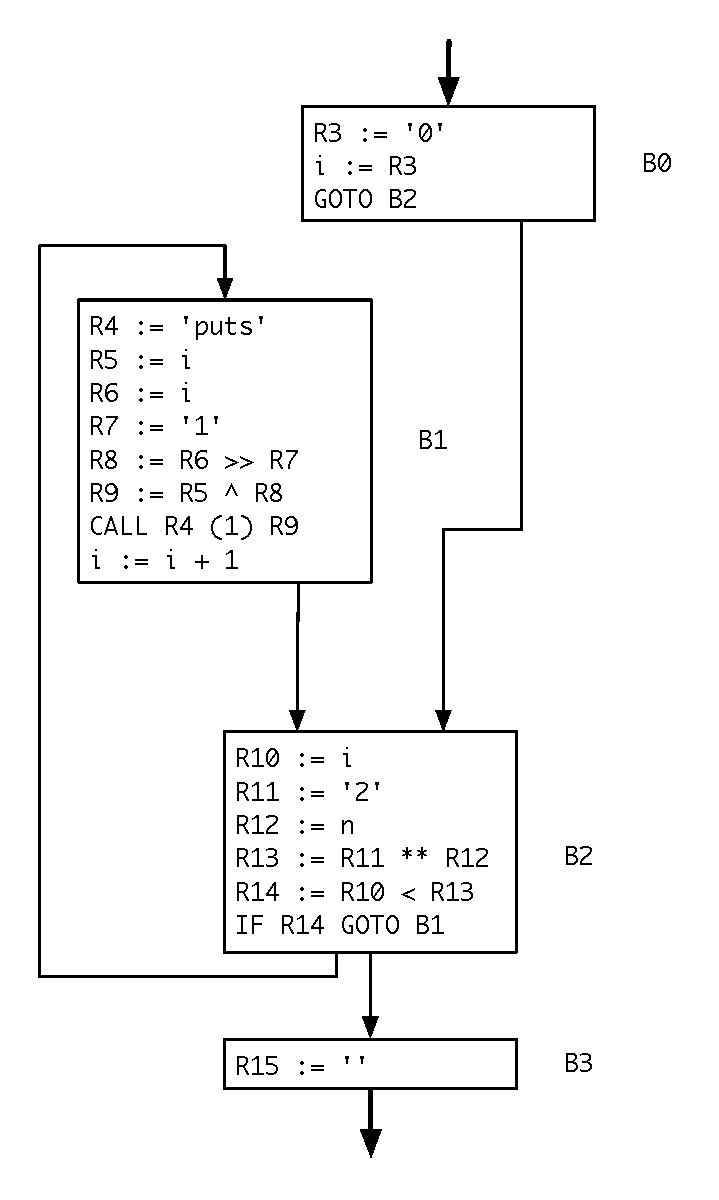
\includegraphics[scale=0.68]{bbs}
  \caption{Blocos básicos e grafo de fluxo de controle construídos \label{bbs}}
\end{figure}

Para se chegar nessa representação foi feita uma espécie de conversão de
máquina virtual baseada em pilha para algo que deveria se assemelhar
com uma máquina de infinitos registradores. Uma pilha temporária é
utilizada para simplificar essa transição, sendo acessada e atualizada
durante a construção de diversas instruções. Também são pré-alocados
registradores virtuais para as variáveis locais. A implementação da
\texttt{Tcl} disponibiliza uma lista dinâmica com todas essas
variáveis locais, incluindo também os parâmetros formais da função,
sendo necessário apenas atribuir índices a elas. O registrador
\verb!R1! está associado ao parâmetro \verb!n!, mas nunca é acessado
diretamente porque o programa exemplo não altera seu valor. Por outro
lado, o \verb!R2! que associa-se a variável local \verb!i! é utilizado
mas foi renomeado (de \verb!R2! para \verb!i!) no desenho acima para
deixar mais claro seu uso.

Verifica-se que há diversas instruções de atribuição que recebem um
valor que se parecem com números, como \verb!'0'! ou \verb!'1'!, mas
que estão sendo representados como strings. Na realidade esses valores
são todos ponteiros para uma estrutura \verb!Tcl_Obj!, podendo assumir
qualquer tipo interno presente na linguagem. Nesse exemplo podemos
assumir, e de fato assim ocorrerá, que todos são inteiros. No caso da
string \verb!'puts'! armazenada no registrador 4 tem-se que ela
servirá como chave em uma tabela hash que possui como valor a
respectiva função (ou não, gerando um erro). O número entre parênteses
na instrução \verb!CALL!
está indicando que haverá 1 parâmetro na chamada e, no caso, este será o
conteúdo de \verb!R9!. A única instrução no bloco de saída B3 indica o
valor de retorno de função -- uma string vazia.

Haviam 55 \textit{bytecodes} sendo utilizados para
representar o código da figura \ref{fig:gray}, e agora 18 quádruplas
são empregadas com o mesmo resultado. Nessa quantidade numérica
superior destaca-se o uso de 9 bytes para representar a instrução
\verb!INST_START_CMD! da \texttt{Tcl}, destinando 4 bytes para contar
a quantidade de instruções à frente que fazem parte desse comando e
possibilitando ao interpretador respeitar limites impostos para certos
recursosatravés de
APIs específicas. Porém, apesar de ser um número menor,
se levarmos em conta o total de bytes contidos em cada quádrupla (de
acordo com as estruturas acima) tem-se que
o consumo de memória é bastante superior. Ao mesmo tempo é possível
observar que muitas delas são passíveis a eliminação, ficando a cargo
de otimizações em etapas futuras.

Um último esclarecimento a respeito da figura \ref{bbs} precisa ser feito.
Os \textit{bytecodes} de desvio emitidos pela \texttt{Tcl} utilizam
operandos que descrevem posições relativas, negativas ou positivas, à
posição atual mas pode-se notar que na
representação utilizada há somente desvios absolutos para blocos
básicos. Para essa tarefa foi feito um mapeamento de cada
\textit{bytecode} para cada bloco básico antes de se construir o
conteúdo deles assumindo que não teriam mais quádruplas do que
\textit{bytecodes}.

\subsection{Mapeamento de alguns \textit{bytecodes} para quádruplas}

XXX.

% XXX Após execução de um procedimento é chamado uma função JIT\_compile
% que agora vive em generic/jit/tclJitCompile.c -- seguindo a nomenclatura
% e estrutura presente na hierarquia do código fonte da Tcl ... XXX

% XXX Fazer ferramenta para encontrar blocos construídos para linguagem
% dot e incluir desenhos aqui. XXX
% ... XXX.

% XXX Mencionar em algum lugar o livro ``Compiladores - Princípios,
% Técnicas e Ferramentas (capítulo 9 ou 8 talvez) XXX

% XXX Descreva nesta seção as partes da proposta já realizadas/implementadas/
% modeladas e já apresente tabelas, gráficos, análise e resultados parciais
% já alcançados, caso existam. XXX


\section{Dificuldades Encontradas}

A primeira dificuldade encontrada foi em relação a aprendizagem
(parcial) do funcionamento da linguagem de programação \texttt{Tcl} --
especificamente a versão 8.5.8 --
que contém mais de 200 mil linhas de código \texttt{C}. Boa parte
desse número de linhas não afeta diretamente a construção desse
compilador, porém uma grande quantidade será ativada
ao longo da execução do código gerado pelo compilador.

A linguagem faz uso de contagem de referências para realizar coleta de
lixo e também compartilha muitos dos valores utilizados. Com isso,
reutilizar objetos \verb!Tcl_Obj! (atualmente no caso da função
\verb!JIT_Compile!) que foram construídos em partes distintas não é tão
simples pois é necessário se ter certeza de que o objeto não será
desalocado enquanto se está trabalhando com ele e, ao mesmo tempo, não
se quer deixar objetos com contagem de referência superior a
necessária. Compartilhar objetos economiza memória mas não simplifica
o uso de objetos alheios, sendo necessário verificar se um objeto
específico é compartilhado ou não antes de, dependendo do uso,
duplicar o mesmo. Não são tarefas tão complexas mas tendem a ser
pontos de erros obscuros em programas não tão curtos e não tão simples.

%Entretanto, a maior dificuldade tem realmente sido conseguir dedicar
%tempo adequado ao trabalho. Sabe-se que a implementação de um
%compilador JIT não é algo simples, ... XXX.


\section{Próximos Passos}

Até o momento pouco foi implementado, porém logo em seguida o que se pretende
fazer é a coleta de tipos. Somente durante a interpretação os
tipos numéricos são descobertos, a representação em \textit{bytecodes}
não possui instruções dedicadas para operandos na pilha com tipos
diferenciados pois todos são inicialmente do tipo \verb!Tcl_Obj! e,
portanto, podem assumir qualquer valores de qualquer forma. Sem essa
coleta fica inviável a
aplicação de até mesmo da otimização de propagação de constante
seguido de empacotamento de constante pois, caso contrário, não
sabemos quais os tipos dos valores em uso.

Seguindo a proposta atual é necessário realizar a construção da forma
SSA após, ou em conjunto, com o passo anterior. Pretende-se seguir o
trabalho de \citeonline{cytron} aqui, obedecendo os algoritmos lá
descritos. Também pretende-se aplicar nesse momento pelo menos algumas
das otimizações que se beneficiam com a representação SSA, tais como
propagação de constantes e eliminação de código morto. Ainda será
avaliado a possibilidade se realizar alocação de registradores
enquanto nessa forma, o trabalho por \citeonline{wimmer_franz} discute
tal tarefa e será a referência base para essa decisão.

Do restante planeja-se seguir com as etapas previstas anteriormente,
refinando-as conforme o projeto avança.


\section{Conclusões}

Compiladores JIT tem sido implementados em máquinas virtuais que demandam
alta performance. Entre as linguagens de programação, \texttt{Java} se
destaca ao ter recebido suficiente atenção ao ponto de empresas e
pesquisadores desenvolverem diversas JVMs com compiladores
dinâmicos que fazem uso de uma variedade de técnicas distintas.

Escolhas adequadas para todas as partes de um compilador JIT tornam
possível o uso de um compilador otimizador em tempo de execução. Esse
texto teve maior foco nas representações intermediárias utilizadas (ou
que serão utilizadas) nesse projeto. Quádruplas para formar blocos
básicos e permitir a construção do grafo de fluxo de controle (CFG)
foi mais discutida aqui, mas também foi mencionado a representação SSA
que inicia-se com a entrada de um CFG. A SSA tem sido aplicada em
diversos compiladores otimizadores, pois permitir aplicar (ao menos)
as otimizações de movimentação de código, propagação de constantes e
eliminação de redundância parcial de forma eficiente.

A conversão de \textit{bytecodes} de uma máquina de pilha para uma
representação na forma de máquina de registradores exige atenção aos
detalhes da semântica implementada na máquina virtual atual da
linguagem. Uma vantagem visível é a capacidade de sintetização que
uma representação baseada em registradores tem sobre uma que faz uso
de pilha. Entretanto, um número reduzido de quádruplas não indica
necessariamente menor consumo de memória do que uma quantidade
superior de \textit{bytecodes}.

% XXX mais ?


% Referências
% Hack: altera \section* para \section temporariamente
\let\stdsection\section
\def\section*#1{\stdsection{#1}}
\bibliography{biblio}
\let\section\stdsection
